\documentclass[landscape,a0paper,fontscale=0.26]{baposter}

\usepackage[T1]{fontenc}
\usepackage[utf8]{inputenc}
\usepackage[english]{babel}
\usepackage{palatino}
\usepackage{multicol}

\usepackage{relsize}

\definecolor{bordercol}{RGB}{89,89,89}
\definecolor{headercol}{RGB}{116,40,60}
\definecolor{opcol}{RGB}{200,0,0}
\definecolor{headerfontcol}{RGB}{255,255,255}
\definecolor{boxcolor}{RGB}{214,214,214}

\graphicspath{{img/}}

\newcommand\opname[2]{{\Large\textbf{\textcolor{opcol}{#1}}}~~~{\large\textbf{#2}}}
\newcommand\op[1]{{\Large\textbf{\textcolor{opcol}{#1}}}}
\newcommand\desc[1]{{\large\textbf{#1}}}

\begin{document}
\typeout{Poster rendering started}
\renewcommand{\arraystretch}{1.4}

\begin{poster}%
  % Poster Options
  {
  	grid=false,
	% Option is left on true though the eyecatcher is not used. The reason is
	% that we have a bit nicer looking title and author formatting in the headercol
	% this way
	eyecatcher=true, 
	borderColor=bordercol,
	headerColorOne=headercol,
	headerColorTwo=headercol,
	headerFontColor=headerfontcol,
	% Only simple background color used, no shading, so boxColorTwo isn't necessary
	boxColorOne=boxcolor,
	headershape=roundedright,
	headerfont=\Large\sf\bf,
	textborder=roundedleft,
	background=none,
	headerborder=open,
  	boxshade=plain
  }
%%% Eye Cacther %%%%%%%%%%%%%%%%%%%%%%%%%%%%%%%%%%%%%%%%%%%%%%%%%%%%%%%%%%%%%%%
{\includegraphics[scale=1.0]{../misc/brachylog_mini_logo.png}}
%%% Title %%%%%%%%%%%%%%%%%%%%%%%%%%%%%%%%%%%%%%%%%%%%%%%%%%%%%%%%%%%%%%%%%%%%%
{\includegraphics[scale=0.8]{../misc/brachylog_logo.png}}
%%% Authors %%%%%%%%%%%%%%%%%%%%%%%%%%%%%%%%%%%%%%%%%%%%%%%%%%%%%%%%%%%%%%%%%%%
{}
%%% Logo %%%%%%%%%%%%%%%%%%%%%%%%%%%%%%%%%%%%%%%%%%%%%%%%%%%%%%%%%%%%%%%%%%%%%%
{\includegraphics[scale=1.0]{../misc/brachylog_mini_logo.png}}


\headerbox{\textsf{Control Flow}}{name=control,column=0,row=0,span=1}{
\begin{center}
\begin{tabular}{cl}
\op{,} & \desc{And}\\
\op{;} & \desc{Or}\\
\op{\textbackslash} & \desc{Backtrack \normalsize{(always false)}}\\
\op{( )} & \desc{Group clauses}\\
\op{!} & \desc{Cut}\\
\op{'} & \desc{Not provable}\\
\op{\textasciitilde} & \desc{Reverse Arguments}\\
\op{:} & \desc{Inline append}\\
\end{tabular}
\end{center}
}

\headerbox{\textsf{Predicates}}{name=predicates,column=0,row=1,span=1,below=control}{
\begin{center}
\begin{tabular}{cl}
\op{\{ \}} & \desc{Inline predicate}\\
\op{\textbackslash n} & \desc{Declare predicate}\\
\op{|} & \desc{New rule}\\
\op{ \&} & \desc{Call predicate}\\
\end{tabular}
\end{center}
}

\headerbox{\textsf{Types and Variables}}{name=types,column=0,row=2,span=1,below=predicates}{
\begin{center}
\begin{tabular}{cl}
\op{?} & \desc{Input of the rule}\\
\op{.} & \desc{Output of the rule}\\
\op{[A-Z]} & \desc{Variables}\\
\op{[I:J]} & \desc{Lists}\\
\op{[]} & \desc{Empty list}\\
\op{"abc"} & \desc{Strings}\\
\op{42} & \desc{Integers}\\
\op{\_25} & \desc{Negative numbers}\\
\op{3.14} & \desc{Floats}\\
\end{tabular}
\end{center}
}

\headerbox{\textsf{Arithmetic}}{name=arithmetic,column=1,row=0,span=1}{
\begin{center}
\begin{tabular}{cl}
\op{+} & \desc{Sum, Absolute value}\\
\op{-} & \desc{Subtract, Negate}\\
\op{*} & \desc{Multiply}\\
\op{/} & \desc{Divide, Inverse}\\
\op{\^{}} & \desc{Power}\\
\op{\%} & \desc{Remainder}\\
\op{\$!} & \desc{Factorial}\\
\op{\$p} & \desc{Prime decomposition}\\
\end{tabular}
\end{center}
}

\headerbox{\textsf{Constraints}}{name=constraints,column=1,row=1,span=1,below=arithmetic}{
\begin{center}
\begin{tabular}{cl}
\op{=} & \desc{Labelize}\\
\op{<} & \desc{Less than}\\
\op{<=} & \desc{Less than or equal}\\
\op{>} & \desc{Greater than}\\
\op{>=} & \desc{Greater than or equal}\\
\op{\#d} & \desc{All different}\\
\op{\#\$} & \desc{Coerce to integer}\\
\op{\#@} & \desc{Coerce to string}\\
\op{\#\#} & \desc{Coerce to list}\\
\end{tabular}
\end{center}
}

\headerbox{\textsf{Strings}}{name=strings,column=1,row=2,span=1,below=constraints}{
\begin{center}
\begin{tabular}{cl}
\op{@l} & \desc{Lowercase}\\
\op{@u} & \desc{Uppercase}\\
\end{tabular}
\end{center}
}

\headerbox{\textsf{Miscellaneous}}{name=miscellaneous,column=1,row=3,span=1,below=strings}{
\begin{center}
\begin{tabular}{cl}
\op{w} & \desc{Write to STDOUT}\\
\op{v} & \desc{Void}\\
\op{z} & \desc{Zip}\\
\end{tabular}
\end{center}
}

\headerbox{\textsf{Math Functions}}{name=functions,column=2,row=0,span=1}{
\begin{center}
\begin{tabular}{cl}
\op{\$e} & \desc{Exponential}\\
\op{\$l} & \desc{Natural logarithm}\\
\op{\$r} & \desc{Square root}\\
\op{\$c} & \desc{cos}\\
\op{\$s} & \desc{sin}\\
\op{\$t} & \desc{tan}\\
\op{\$1} & \desc{arccos}\\
\op{\$2} & \desc{arcsin}\\
\op{\$3} & \desc{arctan}\\
\op{\$4} & \desc{cosh}\\
\op{\$5} & \desc{sinh}\\
\op{\$6} & \desc{tanh}\\
\op{\$7} & \desc{arcosh}\\
\op{\$8} & \desc{arsinh}\\
\op{\$9} & \desc{artanh}\\
\op{\$[} & \desc{Floor}\\
\op{\$]} & \desc{Ceil}\\
\end{tabular}
\end{center}
}

\headerbox{\textsf{Transform}}{name=transform,column=2,row=1,span=1,below=functions}{
\begin{center}
\begin{tabular}{cl}
\op{r} & \desc{Reverse}\\
\op{p} & \desc{Permute}\\
\op{o} & \desc{Order \normalsize{(sort lexicographically)}} \\
\op{g} & \desc{Group \normalsize{(put in a list)}}\\
\op{\$\textbackslash} & \desc{Transpose}\\
\op{\$/} & \desc{Antitranspose}\\
\op{\$(} & \desc{Circular permute left}\\
\op{\$)} & \desc{Circular permute right}\\
\op{@2--9} & \desc{Split in 2--9}\\
\end{tabular}
\end{center}
}

\headerbox{\textsf{Elements}}{name=elements,column=3,row=0,span=1}{
\begin{center}
\begin{tabular}{cl}
\op{h} & \desc{Head \normalsize{(first element)}}\\
\op{b} & \desc{Behead \normalsize{(all but first element)}}\\
\op{t} & \desc{Tail \normalsize{(last element)}} \\
\op{e} & \desc{Enumerate} \\
\op{c} & \desc{Concatenate} \\
\op{d} & \desc{Duplicates} \\
\op{l} & \desc{Length} \\
\op{m} & \desc{Member} \\
\op{s} & \desc{Subset \normalsize{(ordered)}} \\
\op{x} & \desc{Xterminate \normalsize{(strings only for now)}} \\
\end{tabular}
\end{center}
}

\headerbox{\textsf{Meta Predicates}}{name=meta,column=3,row=1,span=1,below=elements}{
\begin{center}
\begin{tabular}{cl}
\op{a} & \desc{Apply}\\
\op{f} & \desc{Findall}\\
\op{i} & \desc{Iterate}\\
\op{\&} & \desc{Call Predicate}\\
\end{tabular}
\end{center}
}

\headerbox{\textsf{Math Constants}}{name=mathcons,column=3,row=2,span=1,below=meta}{
\begin{center}
\begin{tiny}
\begin{tabular}{clccl}
\op{\$A} & \desc{$\frac{1+\sqrt{5}}{2}$} & ~ & \op{\$B} & \desc{$ln(2)$}\\
\op{\$D} & \desc{$ln(10)$} & ~ & \op{\$} & \desc{$e$}\\
\op{\$G} & \desc{$10^9$} & ~ & \op{\$} & \desc{$10^3$}\\
\op{\$M} & \desc{$10^6$} & ~ & \op{\$P} & \desc{$\pi$}\\
\op{\$R} & \desc{$\sqrt{2}$} & ~ & &\\
\end{tabular}
\end{tiny}
\end{center}
}

\headerbox{\textsf{String Constants}}{name=stringcons,column=3,row=3,span=1,below=mathcons}{
\begin{center}
\begin{tiny}
\begin{tabular}{clcl}
\op{@A} & \desc{\small{Alphabet}} &  \op{@C} & \desc{\small{Consonants}}\\
\op{@D} & \desc{\small{Cons. var.}} & \op{@H} & \desc{\small{"Hello, World!"}}\\
\op{@N} & \desc{\small{"\textbackslash n"}} & \op{@P} & \desc{\small{Printable ASCII}}\\
\op{@Q} & \desc{\small{"@Qw"}} & \op{@S} & \desc{\small{" "}}\\
\op{@T} & \desc{\small{"\textbackslash t"}} & \op{@V} & \desc{\small{Vowels}}\\
\op{@W} & \desc{\small{Vow. var.}} & \op{@Z} & \desc{\small{Rev. Alphabet}}\\
\end{tabular}
\end{tiny}
\end{center}
}

\end{poster}  

\end{document}